\documentclass[tikz,border=8pt]{standalone}
% Shared look for every TikZ diagram. Load with % Shared look for every TikZ diagram. Load with % Shared look for every TikZ diagram. Load with \input{../../tools/tikz-style.tex}
\usepackage[T1]{fontenc}
\usepackage{lmodern}
\renewcommand{\sfdefault}{lmr}  % diagrams use the same serif as the text
\usetikzlibrary{arrows.meta, positioning, shapes.geometric, calc, fit, backgrounds}
\definecolor{cblue}{HTML}{4C78A8}
\definecolor{corange}{HTML}{F58518}
\definecolor{cgreen}{HTML}{54A24B}
\definecolor{cred}{HTML}{E45756}
\definecolor{cpurple}{HTML}{B279A2}
\definecolor{cgrey}{HTML}{6B6B6B}
\tikzset{
  every picture/.style={font=\sffamily, line width=1.2pt},
  box/.style={draw=#1, fill=#1!12, rounded corners=4pt, align=center, inner sep=7pt, minimum height=1.1cm},
  box/.default=cgrey,
  arrow/.style={-{Stealth[length=3mm]}, draw=cgrey, line width=1.4pt},
  title/.style={font=\sffamily\bfseries\Large},
  note/.style={font=\sffamily\small, text=cgrey, align=center},
}
\AtBeginDocument{\hyphenpenalty=10000 \exhyphenpenalty=10000}

\usepackage[T1]{fontenc}
\usepackage{lmodern}
\renewcommand{\sfdefault}{lmr}  % diagrams use the same serif as the text
\usetikzlibrary{arrows.meta, positioning, shapes.geometric, calc, fit, backgrounds}
\definecolor{cblue}{HTML}{4C78A8}
\definecolor{corange}{HTML}{F58518}
\definecolor{cgreen}{HTML}{54A24B}
\definecolor{cred}{HTML}{E45756}
\definecolor{cpurple}{HTML}{B279A2}
\definecolor{cgrey}{HTML}{6B6B6B}
\tikzset{
  every picture/.style={font=\sffamily, line width=1.2pt},
  box/.style={draw=#1, fill=#1!12, rounded corners=4pt, align=center, inner sep=7pt, minimum height=1.1cm},
  box/.default=cgrey,
  arrow/.style={-{Stealth[length=3mm]}, draw=cgrey, line width=1.4pt},
  title/.style={font=\sffamily\bfseries\Large},
  note/.style={font=\sffamily\small, text=cgrey, align=center},
}
\AtBeginDocument{\hyphenpenalty=10000 \exhyphenpenalty=10000}

\usepackage[T1]{fontenc}
\usepackage{lmodern}
\renewcommand{\sfdefault}{lmr}  % diagrams use the same serif as the text
\usetikzlibrary{arrows.meta, positioning, shapes.geometric, calc, fit, backgrounds}
\definecolor{cblue}{HTML}{4C78A8}
\definecolor{corange}{HTML}{F58518}
\definecolor{cgreen}{HTML}{54A24B}
\definecolor{cred}{HTML}{E45756}
\definecolor{cpurple}{HTML}{B279A2}
\definecolor{cgrey}{HTML}{6B6B6B}
\tikzset{
  every picture/.style={font=\sffamily, line width=1.2pt},
  box/.style={draw=#1, fill=#1!12, rounded corners=4pt, align=center, inner sep=7pt, minimum height=1.1cm},
  box/.default=cgrey,
  arrow/.style={-{Stealth[length=3mm]}, draw=cgrey, line width=1.4pt},
  title/.style={font=\sffamily\bfseries\Large},
  note/.style={font=\sffamily\small, text=cgrey, align=center},
}
\AtBeginDocument{\hyphenpenalty=10000 \exhyphenpenalty=10000}

\begin{document}
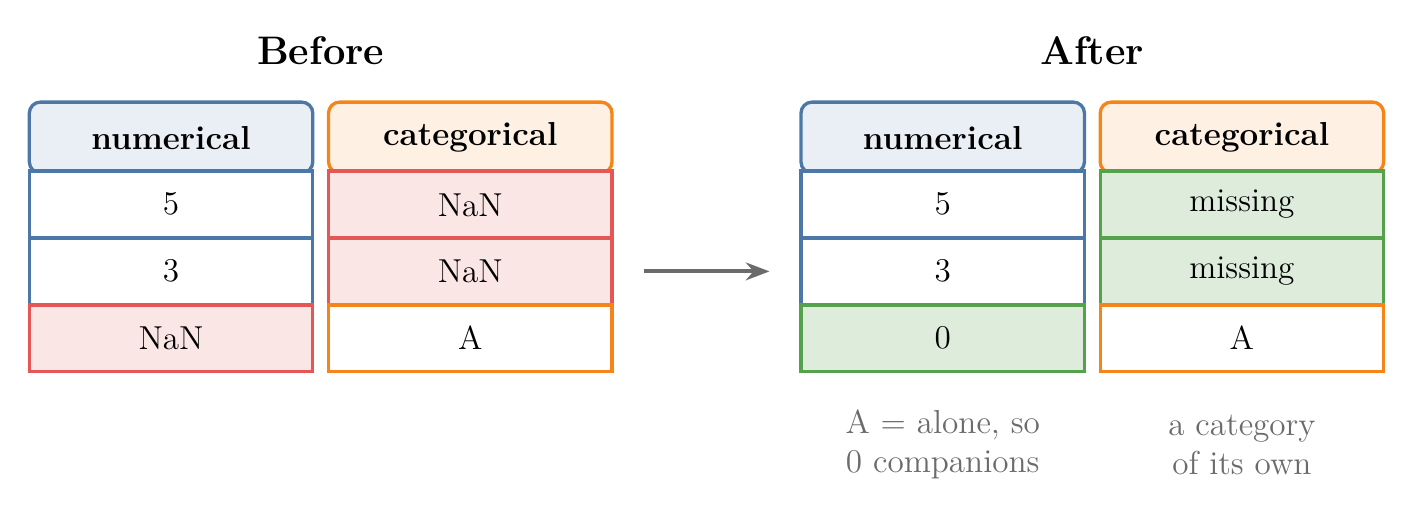
\begin{tikzpicture}[every node/.append style={font=\sffamily\large}]
\tikzset{note/.style={font=\sffamily\large, text=cgrey, align=center}}
  \tikzset{cl/.style={draw=#1, fill=white, minimum width=3.6cm, minimum height=0.85cm},
           hd/.style={box=#1, minimum width=3.6cm, minimum height=0.9cm, inner sep=3pt},
           gap/.style={draw=cred, fill=cred!15, minimum width=3.6cm, minimum height=0.85cm},
           fix/.style={draw=cgreen, fill=cgreen!20, minimum width=3.6cm, minimum height=0.85cm}}
  \node[title] at (1.9,1.1) {Before};
  \node[hd=cblue] at (0,0) {\textbf{numerical}};
  \node[hd=corange] at (3.8,0) {\textbf{categorical}};
  \node[cl=cblue] at (0,-0.85) {5};   \node[gap] at (3.8,-0.85) {NaN};
  \node[cl=cblue] at (0,-1.7) {3};    \node[gap] at (3.8,-1.7) {NaN};
  \node[gap] at (0,-2.55) {NaN};      \node[cl=corange] at (3.8,-2.55) {A};
  \draw[arrow] (6.0,-1.7) -- (7.6,-1.7);
  \begin{scope}[xshift=9.8cm]
  \node[title] at (1.9,1.1) {After};
  \node[hd=cblue] at (0,0) {\textbf{numerical}};
  \node[hd=corange] at (3.8,0) {\textbf{categorical}};
  \node[cl=cblue] at (0,-0.85) {5};   \node[fix] at (3.8,-0.85) {missing};
  \node[cl=cblue] at (0,-1.7) {3};    \node[fix] at (3.8,-1.7) {missing};
  \node[fix] at (0,-2.55) {0};        \node[cl=corange] at (3.8,-2.55) {A};
  \end{scope}
  \node[note, text width=3.6cm] at (9.8,-3.9) {A = alone, so 0 companions};
  \node[note, text width=3.6cm] at (13.6,-3.9) {a category of its own};
\end{tikzpicture}
\end{document}
